\documentclass{article}
\usepackage[T1]{fontenc}
\usepackage{lmodern}
\usepackage[ngerman]{babel}
\usepackage{graphicx}

\title{ASIC Implementierung einer Zweidimensionalen Flugbahnberechnung mittels Heun-Verfahren und Stokes Reibung}
\author{Julius Gilka-Bötzow}
\date{WiSe 2021-22}

% Für die Code Blöcke
\usepackage{listings, listings-rust}
\usepackage{xcolor}
\definecolor{codegreen}{rgb}{0,0.6,0}
\definecolor{codegray}{rgb}{0.5,0.5,0.5}
\definecolor{codepurple}{rgb}{0.58,0,0.82}
\definecolor{backcolour}{rgb}{0.95,0.95,0.92}
\lstdefinestyle{mystyle}{
    backgroundcolor=\color{backcolour},
    commentstyle=\color{codegreen},
    keywordstyle=\color{magenta},
    numberstyle=\tiny\color{codegray},
    stringstyle=\color{codepurple},
    basicstyle=\ttfamily\footnotesize,
    breakatwhitespace=false,
    breaklines=true,
    captionpos=b,
    keepspaces=true,
    numbers=left,
    numbersep=5pt,
    showspaces=false,
    showstringspaces=false,
    showtabs=false,
    tabsize=2
}
\lstset{style=mystyle}


\begin{document}

    \begin{titlepage}
        \maketitle
    \end{titlepage}

    \begin{abstract}
        In diesem Beleg wird der Entwurfs- und Testprozess eines Application-specific integrated circuit (ASIC)
        dargestellt. Entstanden ist das Ganze als Praktikum im Fach Schaltkreis- und Systementwurf an der TU Dresden.
    \end{abstract}


    \newpage
    \tableofcontents
    \newpage


    \section{Aufgabenstellung}

    Der Rahmen für die mir selbst gestellte Aufgabe ist wie folgt.

    Ich wurde von einem Rüstungsunternehmen gebeten einen ASIC für schnelle Flugbahnberechnung zu entwerfen.
    Dieser soll in den Computer eines Artillerie-Geschützes eingebaut werden.

    \newblock

    Da es sich um das Militär als Kunden handelt, sind Kosten und somit Fläche keine Limitation.
    Fokus liegt auf der Geschwindigkeit, Genauigkeit und Energieeffizienz, weil es möglicherweise mit einer
    Batterie betrieben wird.

    \newblock

    Damit der Chip mit dem Rest des Systems funktionieren kann, gibt es folgende E/A-Vorgaben.

    Eingegeben werden eine Startposition und -geschwindigkeit (jeweils mit x und y Koordinaten), der Radius
    und die Masse des Geschosses, sowie die Länge der Zeitschritte um die Berechnungsgenauigkeit anpassen zu können.

    Ausgegeben wird eine Liste von Werten mit x und y Postionen, die in einen dem ASIC externen Speicher zur späteren
    weiterverarbeitung gespeichert werden. Der Zeitstempel ist implizit in der Stelle des
    Elementes im Speicher.

    \newblock

    Um diese Aufgabe zu lösen habe ich zuerst eine Implementierung in Rust geschrieben und diese Anschließend
    überarbeitet um sie auf einen ASIC übertragen zu können.

    \section{Programmablauf}

    \subsection{Initiale Version}

    Das Programm nutzt den Heun-Algorithmus, der Schrittweise von einem Startwert und seiner Ableitung eine Kurve aus
    Punkten entwickelt.
    Diesen habe ich überlagert mit dem Gesetzt von Stokes um die Luftreibung zu simulieren.

    \newblock

    In der ersten Version (Listing \ref{lst:Codeblock initial}) sind keine Optimierungen vorgenommen. Sowohl für die Anzahl
    der Operationen als auch die Umsetzbarkeit für ASICs.

    \newpage

    \begin{lstlisting}[language=Rust, caption={Initialer Code.}, label=lst:Codeblock initial]
        // Constants will be read from memory
        const PI: f64 = 3.142;
        const VISC: f64 = 0.000018215;
        // Dynamic Viscosity of air at 20 degree Celsius in kg/(m*s)

        // position: tuple of x,y in meters
        // velocity: tuple of x,y in meters per second
        // radius: value in meters
        // delta_t: value in seconds for timesteps
        // mass: value in kilogram
        // return: Vec of tuple of pos_x, pos_y, vel_x, vel_y, time
        pub fn get_list(position: (f64, f64), velocity: (f64, f64),
            radius: f64, delta_t: f64, mass: f64) -> Vec<(f64, f64, f64, f64, f64)>{
            // Set initial values
            let mut rx = position.0;
            let mut ry = position.1;
            let mut vx = velocity.0;
            let mut vy = velocity.1;
            let mut t = 0.0;
            let dt = delta_t;
            let gx = 0.0;
            let gy = -9.81;

            // Save initial values in new Vector
            let mut vec = vec![(rx, ry, vx, vy, t)];
            loop {
                // Calculate next velocity with gravity and stokes
                let next_vx = vx + (gx -6.0*PI*radius*VISC * vx / mass)*dt;
                let next_vy = vy + (gy -6.0*PI*radius*VISC * vy / mass)*dt;
                // Calculate next position with median of speeds
                let newrx = rx + (vx + next_vx)/2.0 * dt;
                let newry = ry + (vy + next_vy)/2.0 * dt;
                // Assign new values
                t += dt;
                rx = newrx;
                ry = newry;
                vx = next_vx;
                vy = next_vy;
                // break when reaching the "ground" aka y==0
                if ry < 0.0{
                    break;
                }
                vec.push((rx, ry, vx, vy, t));
            }
            return vec;
        }
    \end{lstlisting}

    \newpage

    Zu beachten ist hierbei, dass ist den Vector anschließend in eine Textdatei geschrieben habe und diese anschließend
    mit R geplotted. Dazu ist die Zeit als weitere Ausgabe notwendig.

    Der Zweck des Plottens war es zu sehen ob der Algorithmus das erwartete Resultat bringt und ob die Reibung einen
    merkbaren Einfluss hat oder vernachlässigt werden kann.



    \begin{figure}[!htbp]
        \includegraphics[width=\textwidth]{../Ballistiken/PlotExports/Ortsänderung mit 1000.png}
        \caption{Plot des Initialen Algorithmus.}
        \label{Ortsplot initial}
    \end{figure}


    \subsection{Verbesserte Version}

    Anschließend habe ich einige Optimierungen vorgenommen.
    Als erstes habe ich Zeile Code aufgeteilt um jeweils nur eine Operation pro Zeile zu haben.
    Dabei ist mir aufgefallen, dass einige Operationen vor den Loop gebracht können werden, wenn man die Gleichungen
    etwas umstellt. Dadurch entstehen mehr Operationen am Start aber pro Loop-Durchlauf werden Operationen
    gespart.

    \newblock

    Nach einigen Experimenten mit Festkommadarstellungen um Platz zu sparen, habe ich mich entschieden bei der floating
    point Darstellung zu bleiben. Hauptgrund war die Kundenvorgabe der Genauigkeit aber auch die einfachere Umsetzung
    war ein Faktor.

    \newpage

    \begin{lstlisting}[language=Rust, caption={Optimierter Code.}, label=lst:Codeblock besser]
        const PI: f64 = 3.142;
        const VISC: f64 = 0.000018215;

        const STOKES: f64 = 0.000343345;

        pub fn get_list(position: (f64, f64), velocity: (f64, f64),
                        radius: f64, delta_t: f64, mass: f64)
                        -> Vec<(f64, f64, f64, f64, f64)>{

            let mut rx = position.0;
            let mut ry = position.1;
            let mut vx = velocity.0;
            let mut vy = velocity.1;
            let mut t = 0.0;

            // Helpful "constants"
            let stokes_const_1 = STOKES * radius;
            let stokes_const_2 = stokes_const_1/mass;
            let stokes_const = stokes_const_2 * delta_t;
            let earth_speed_y = -9.81 * delta_t;
            let half_step = delta_t/2.0;

            // Save initial values in new Vector
            let mut vec = vec![(rx, ry, vx, vy, t)];
            loop {
                // Calculate next velocity with gravity and stokes
                let next_vx_1 = stokes_const * vx;
                let next_vx = vx - next_vx_1;
                let next_vy_1 = vy + earth_speed_y;
                let next_vy_2 = stokes_const * vy;
                let next_vy = next_vy_1 - next_vy_2;
                // Calculate next position with median of speeds
                let newrx_1 = vx + next_vx;
                let newrx_2 = newrx_1 * half_step;
                let newrx = rx + newrx_2;
                let newry_1 = vy + next_vy;
                let newry_2 = newry_1 * half_step;
                let newry = ry + newry_2;
                // Assign new values
                t += delta_t;
                rx = newrx;
                ry = newry;
                vx = next_vx;
                vy = next_vy;
                // break when reaching the "ground" aka y==0
                if ry < 0.0{
                    break;
                }
                vec.push((rx, ry, vx, vy, t));
            }
            return vec;
        }
    \end{lstlisting}

    \newpage

    Um zu überprüfen ob der Code das selbe verhalten hat, habe ich das Ergebnis wieder als Plot dargestellt.

    \begin{figure}[!htbp]
        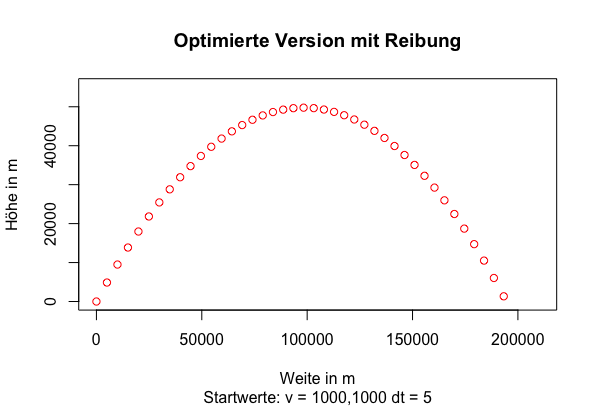
\includegraphics[width=\textwidth]{../Ballistiken/PlotExports/Optimiert.png}
        \caption{Plot des Optimierten Algorithmus.}
        \label{Ortsplot initial}
    \end{figure}

    Da das Verhalten des Optimierten Algorithmus das gleiche ist das des initialen ist, nutze ich den
    optimierten Code als Grundlage für das weitere Vorgehen. Namentlich den DFG im nächsten Abschnitt.


    \section{Datenpfadarchitektur}

    \subsection{Datenflussgraph}

    Der DFG ist in aufgrund seiner Länge auf zwei Seiten verteilt.
    Die erste Seite (Abbildung \ref{DFG1}), zeigt alles vor Anfang des Loops,
    die zweite (Abbildung \ref{DFG2}) alles im Loop.

    \begin{figure}
        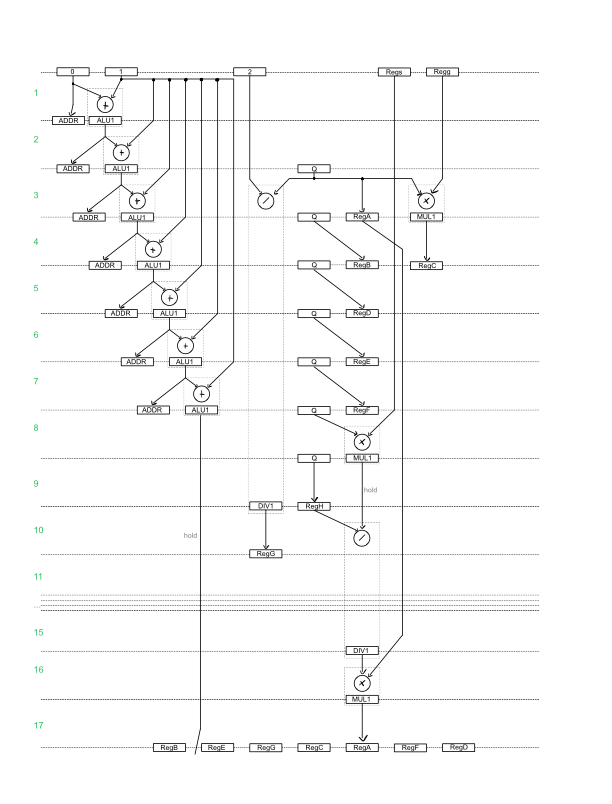
\includegraphics[width=\textwidth]{../Diagramme/Datenflussdiagramm/DFG_VorerstFinal_S1.png}
        \caption{Datenflussgraph vor dem Loop}
        \label{DFG1}
    \end{figure}

    \begin{figure}
        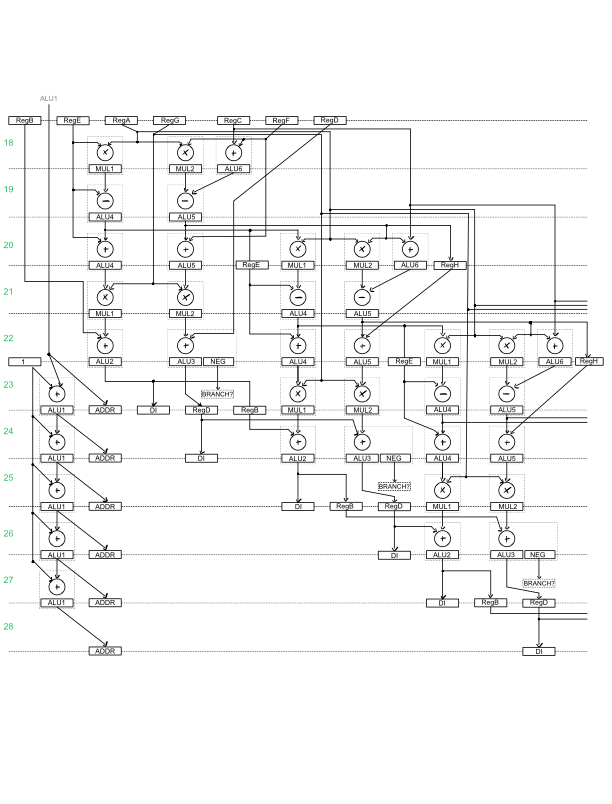
\includegraphics[width=\textwidth]{../Diagramme/Datenflussdiagramm/DFG_VorerstFinal_S2.png}
        \caption{Datenflussgraph im Loop}
        \label{DFG2}
    \end{figure}

    \newpage
    
    \subsection{Register-Transfer-Folge}

    Diese erste Version der RT-Folge besteht aus LOAD, PREP, LOOP, FULL und END.
    \begin{itemize}
        \item LOAD lädt am Anfang die nötigen Daten aus dem Speicher.
        \item PREP bezeichnet die Takte nach dem Lade aber vor dem Beginn des Loop.
        \item LOOP meint den Anfang des Loops, wenn die Pipeline noch nicht voll gelaufen ist.
        \item FULL sind zwei abwechselnde States, bei denen die Pipeline schon voll gelaufen ist.
        \item END ist ein simpler Endzustand.
    \end{itemize}

    \begin{figure}
        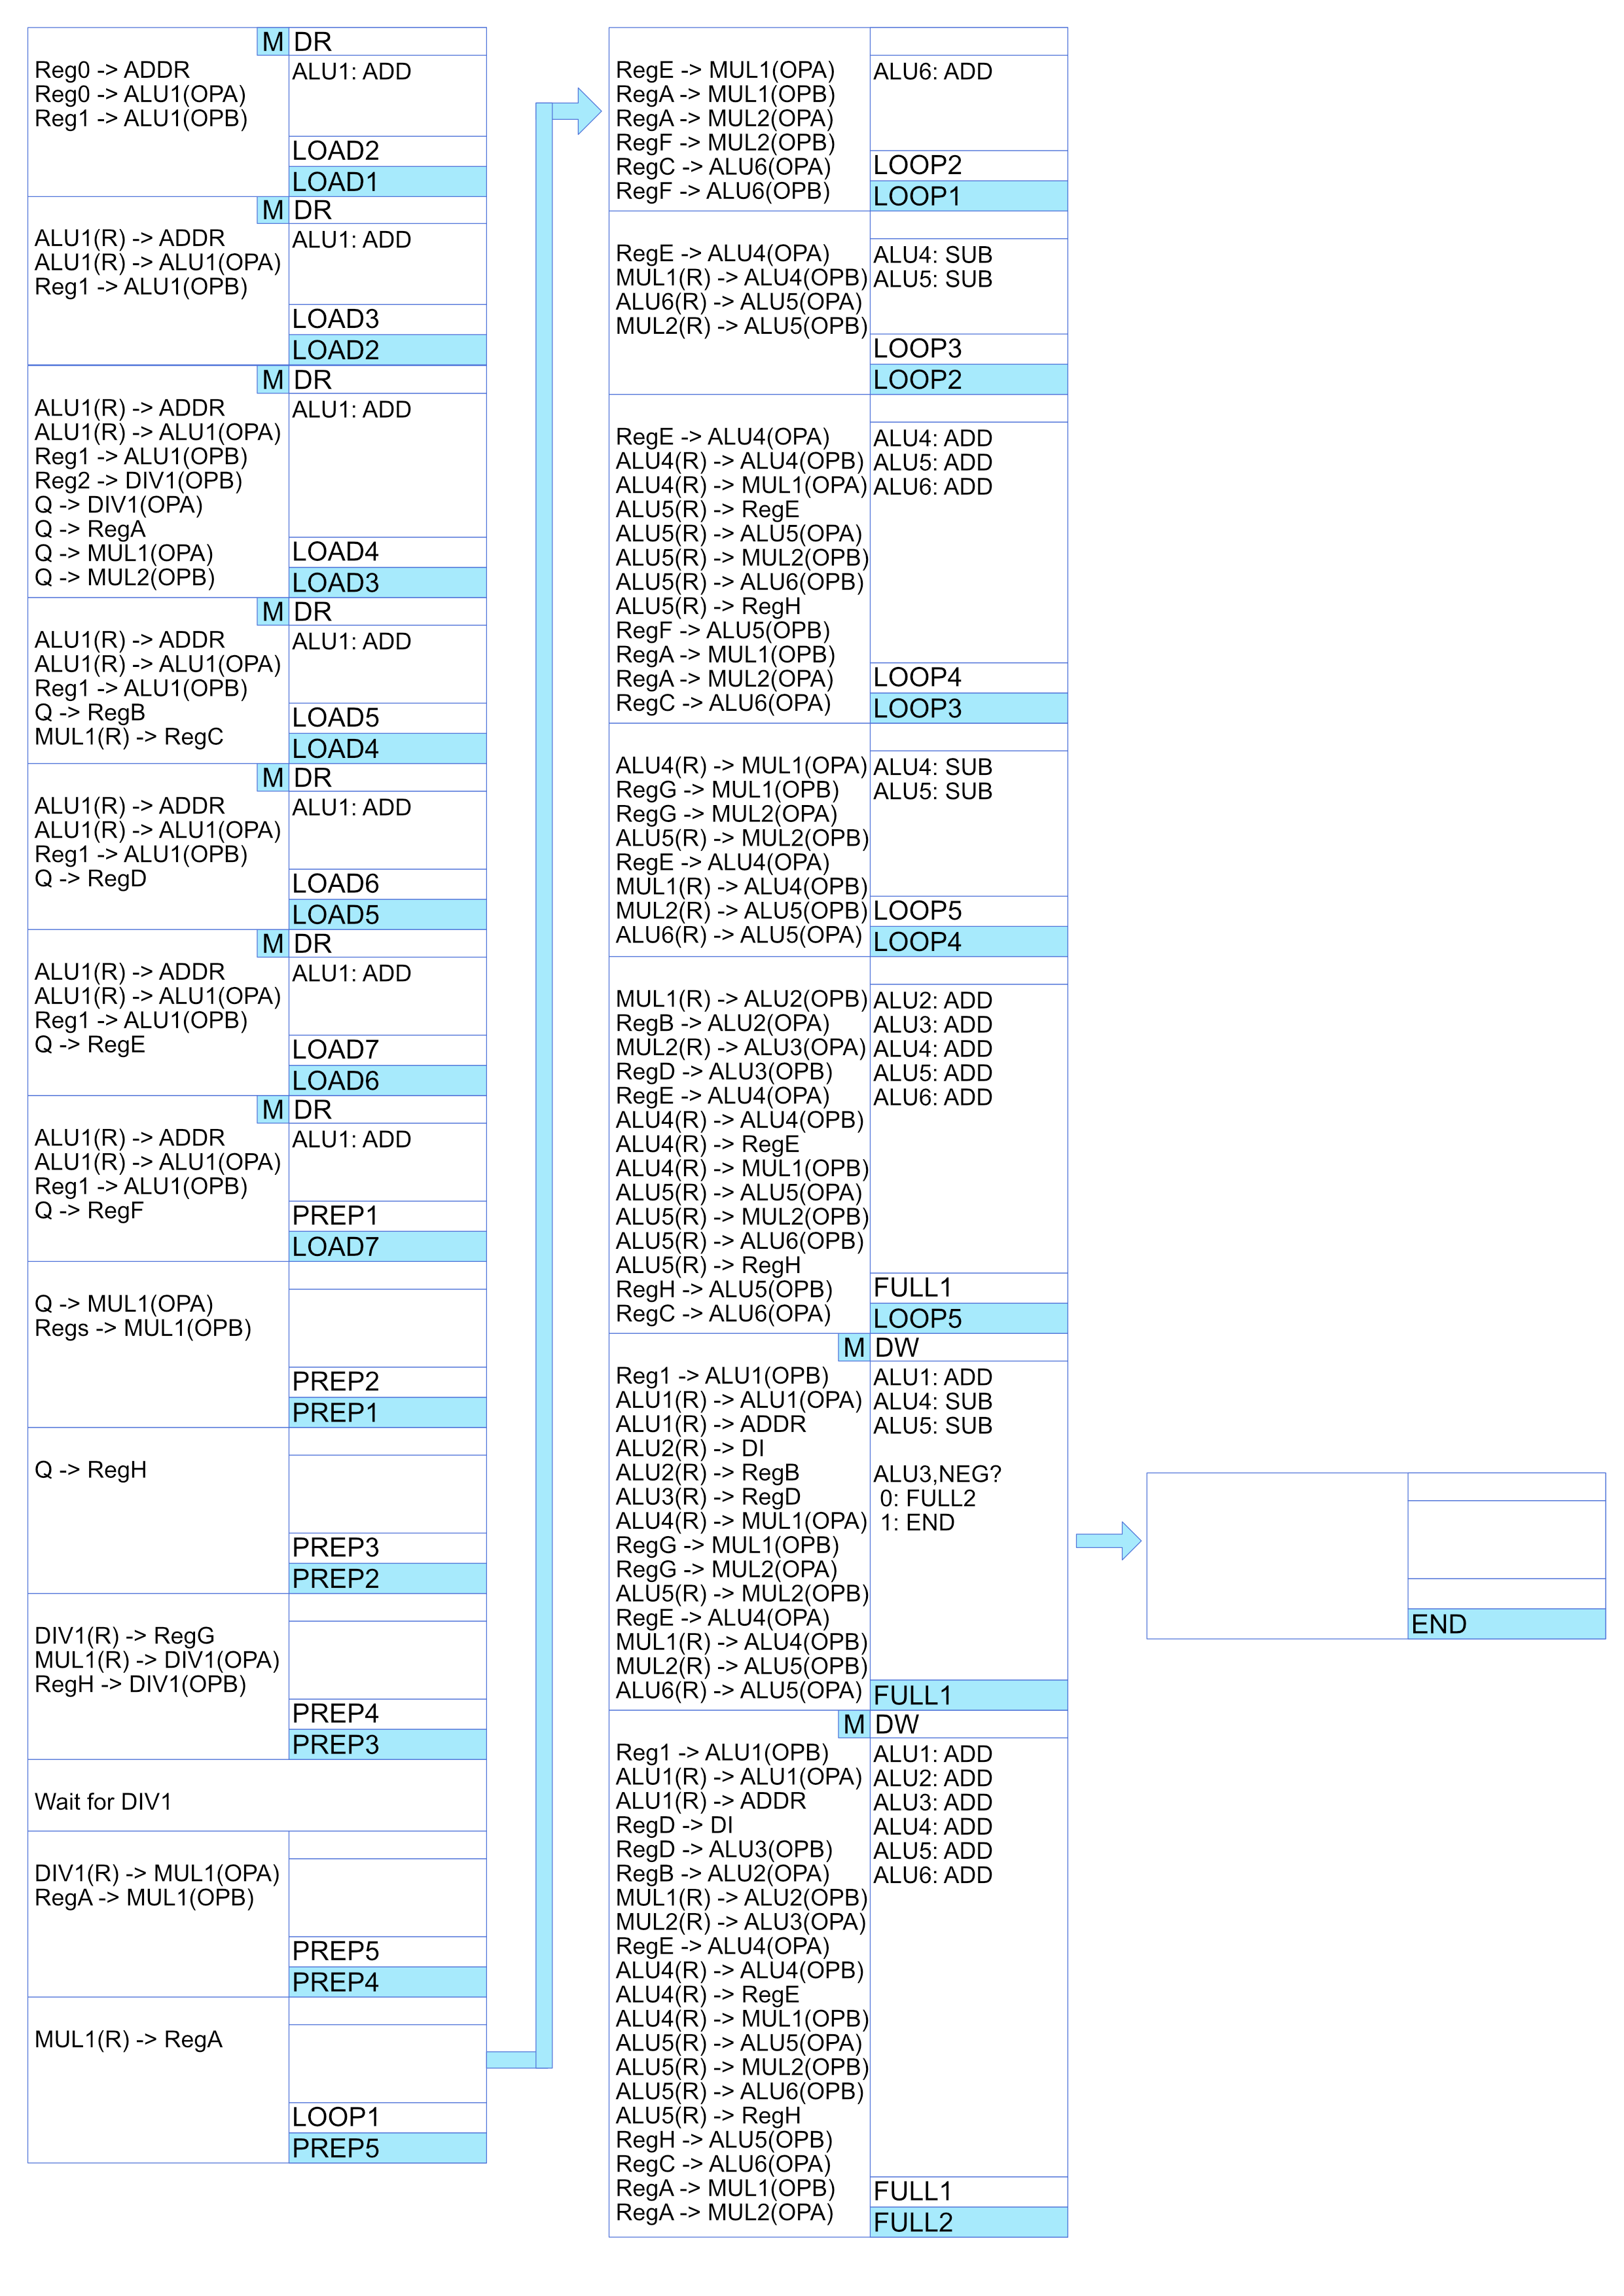
\includegraphics[width=\textwidth]{../Diagramme/RegisterTransferfolge/RegisterTransferFolgeKomplett.png}
        \caption{Register-Transfer-Folge}
        \label{RT-Folge}
    \end{figure}

    \subsection{Datenpfadarchitektur}

    Aus der Registertransferfolge habe ich erkennen können, dass diese Schaltung 12 Busse benötigt.
    Diese habe ich von A bis L benannt.

    % Erste Version einfügen

\end{document}